\documentclass[12pt, letterpaper]{article}
\usepackage[utf8]{inputenc} % utf-8 standard Encoding Text
\usepackage[spanish]{babel} % Permit Spanish Text
\usepackage{multirow} % Use Text Multirow  with custom size
\usepackage{graphicx} % Use to set graphics
\usepackage{tabularx,ragged2e,booktabs,caption,anyfontsize,rcsinfo} % provides a column type which expands to fill the specified width of the table, text alignment,
\usepackage[section]{placeins}
\usepackage{verbatim} % coments but not show
\usepackage{hyperref} % Reference
\usepackage{import} % Import other tex files
\usepackage{changes} % Show differents Changes with color by User 
\usepackage{lipsum} % ?????
\usepackage[yyyymmdd,hhmmss]{datetime} % date time format
\usepackage{pifont}


\addto\captionsspanish{\def\listofchangesname{List of changes}}
\addto\captionsspanish{\def\summaryofchangesname{Changes}}
\addto\captionsspanish{\def\changesaddname{Added}}
\addto\captionsspanish{\def\changesdeletename{Deleted}}
\addto\captionsspanish{\def\changesreplacename{Replaced}}
\addto\captionsspanish{\def\changesauthorname{Author}}
\addto\captionsspanish{\def\changesanonymousname{anonymous}}
\addto\captionsspanish{\def\changesnoloc{List of changes is available after the next \LaTeX\ run.}}
\addto\captionsspanish{\def\changesnosoc{Summary of changes is available after the next \LaTeX\ run.}}


\providecommand{\versionnumber}{3.0.1}
\title{Manual Modulo Videowidget \\\normalsize Version \versionnumber}
\author{ Operador de Computo: Adrián Romero Vargas \copyright~2015 Pengostores }
\date{\today}



\begin{document}


\begin{titlepage}

\begin{figure}[htp]
\centering

\includegraphics[width=15cm]{logo-pengo}
\end{figure}

\currenttime

\par


\begin{comment}
Este paso solo funciona si .....  Y no debe Verse
\end{comment}


\begin{center}
{\huge Pengo Manual}
\end{center}


\centering
{\fontsize{1cm}{1cm}\selectfont Modulo Pengo Videowidget 
\par}



\end{titlepage}

\tableofcontents{}

\listoftables{}

\listoffigures

\maketitle

\section{Primeros Pasos}
 
{\centering

Este es un modulo que no depende de ningún otro.



}


Algo no debe estar bien. \added{ \ding{51}Cambiar Esto.}

La funcionalidad de este modulo es mostrar un vídeo youtube en un CMS,Bloque estático 

\begin{center}
\captionof{table}{Primera tabla}
\begin{tabular}{ |p{3cm}||p{3cm}|p{3cm}|p{3cm}|  }
 \hline
 \multicolumn{4}{|c|}{Video en Internet} \\
 \hline
 Video Proveedor & Formato & Ventaja & Audiencia\\
 \hline
  Youtube   & FLV,MPG4,VMV & Muy Popular G&  total 100\% \\
  Vimeo&   FLV,MPG4   & No tan Popular   &  total 40\%  \\
  Tutv & FLV & Solo Hispanoamerica &  total 20\% \\
  Google Video  &Solo en Noticias & DZA&  012\\
 Dialymotion& FLV,MPG4  & Independientes & Europa Francia\\
 Facebook Videos& FLV,MPG4 & En facebook Licencia & Solo Facebook ?\\
 Megavideo& FLV,MG4,vorbis & Conodido por Mega Upload& Solo usuarios antes 2013\\
 \hline
\end{tabular}
\end{center}
 
\section{Pasos para Configurarlo}
 
Todos los pasos para configurarlo se encuentran aquí:

\subsection{Paso 1}

En el Paso Uno veremos

\begin{figure}[htp]
\centering
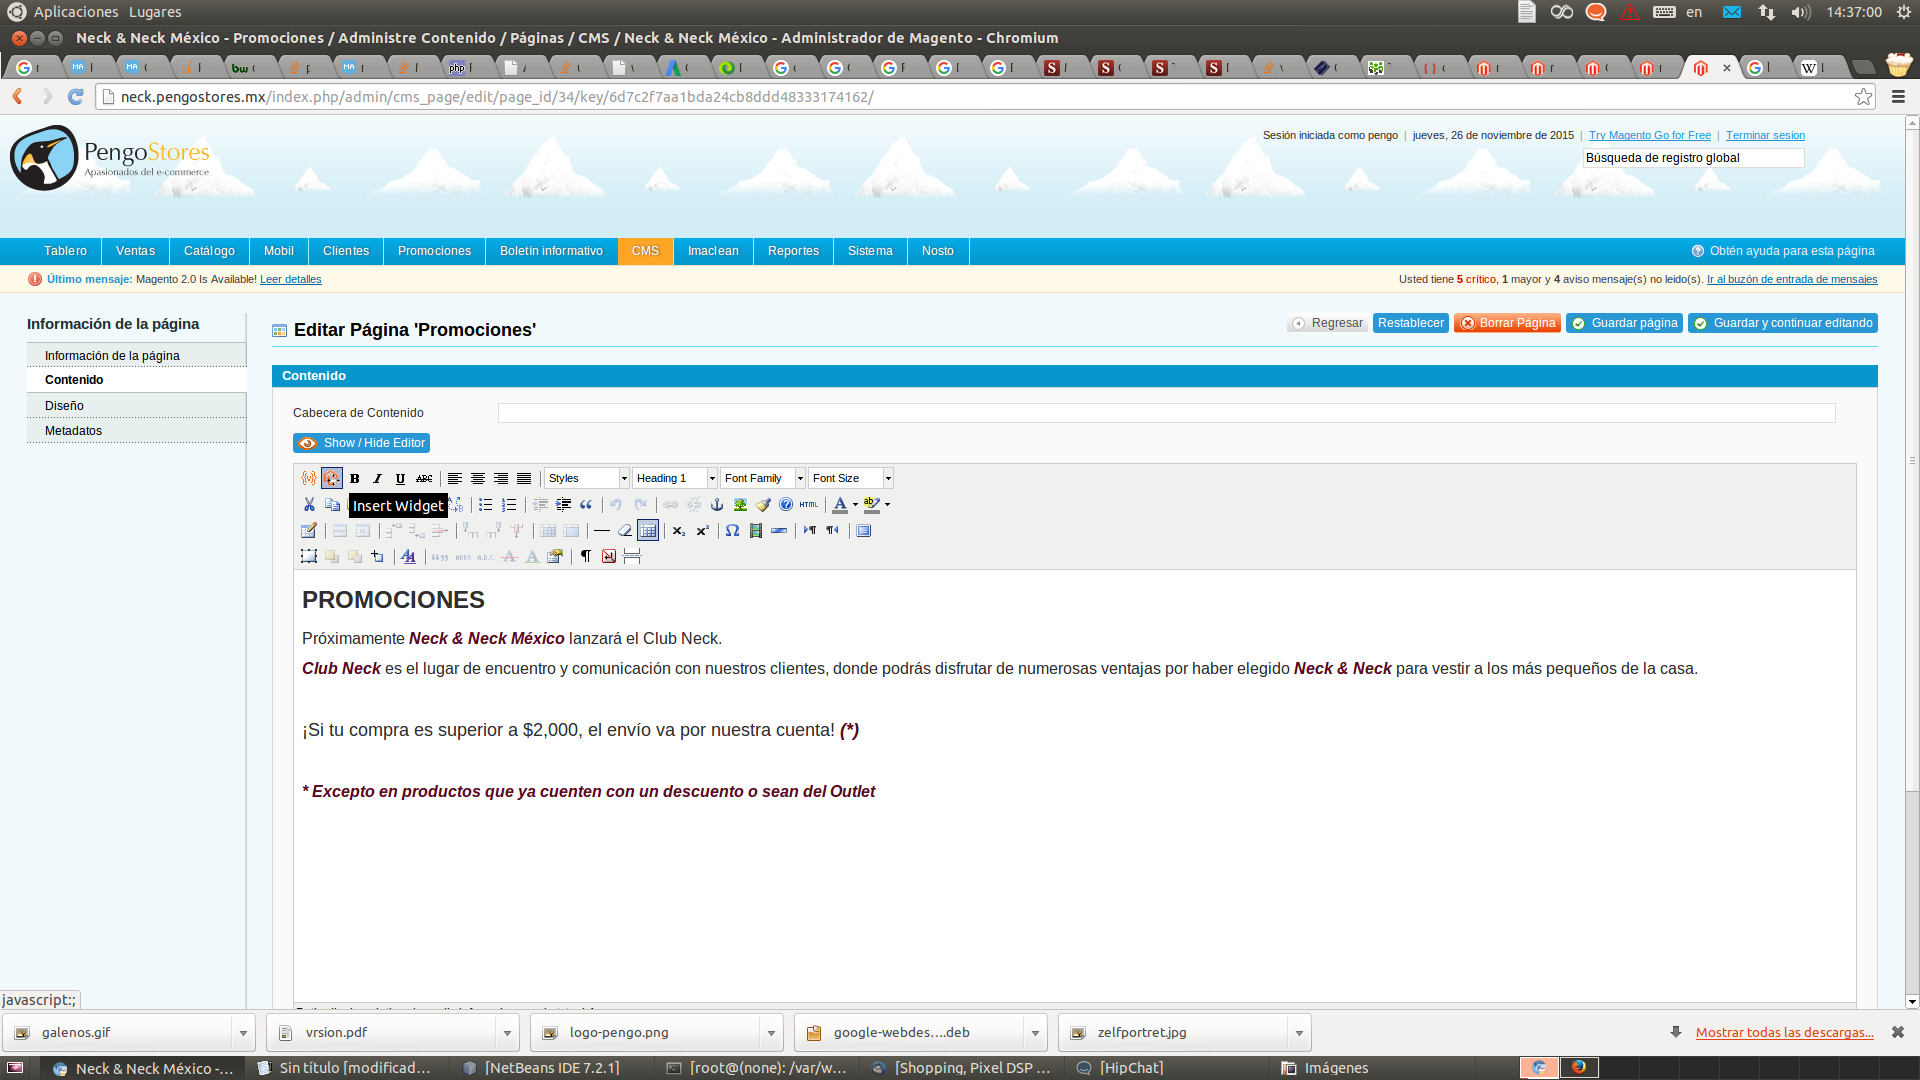
\includegraphics[width=16cm]{widget00}
\caption{pantalla Inicio}
\label{fig:simple}
\end{figure}

Para el final del paso debemos

\subsection{Paso 2}

{\centering
Durante el paso 2

\begin{figure}[htp]
\centering
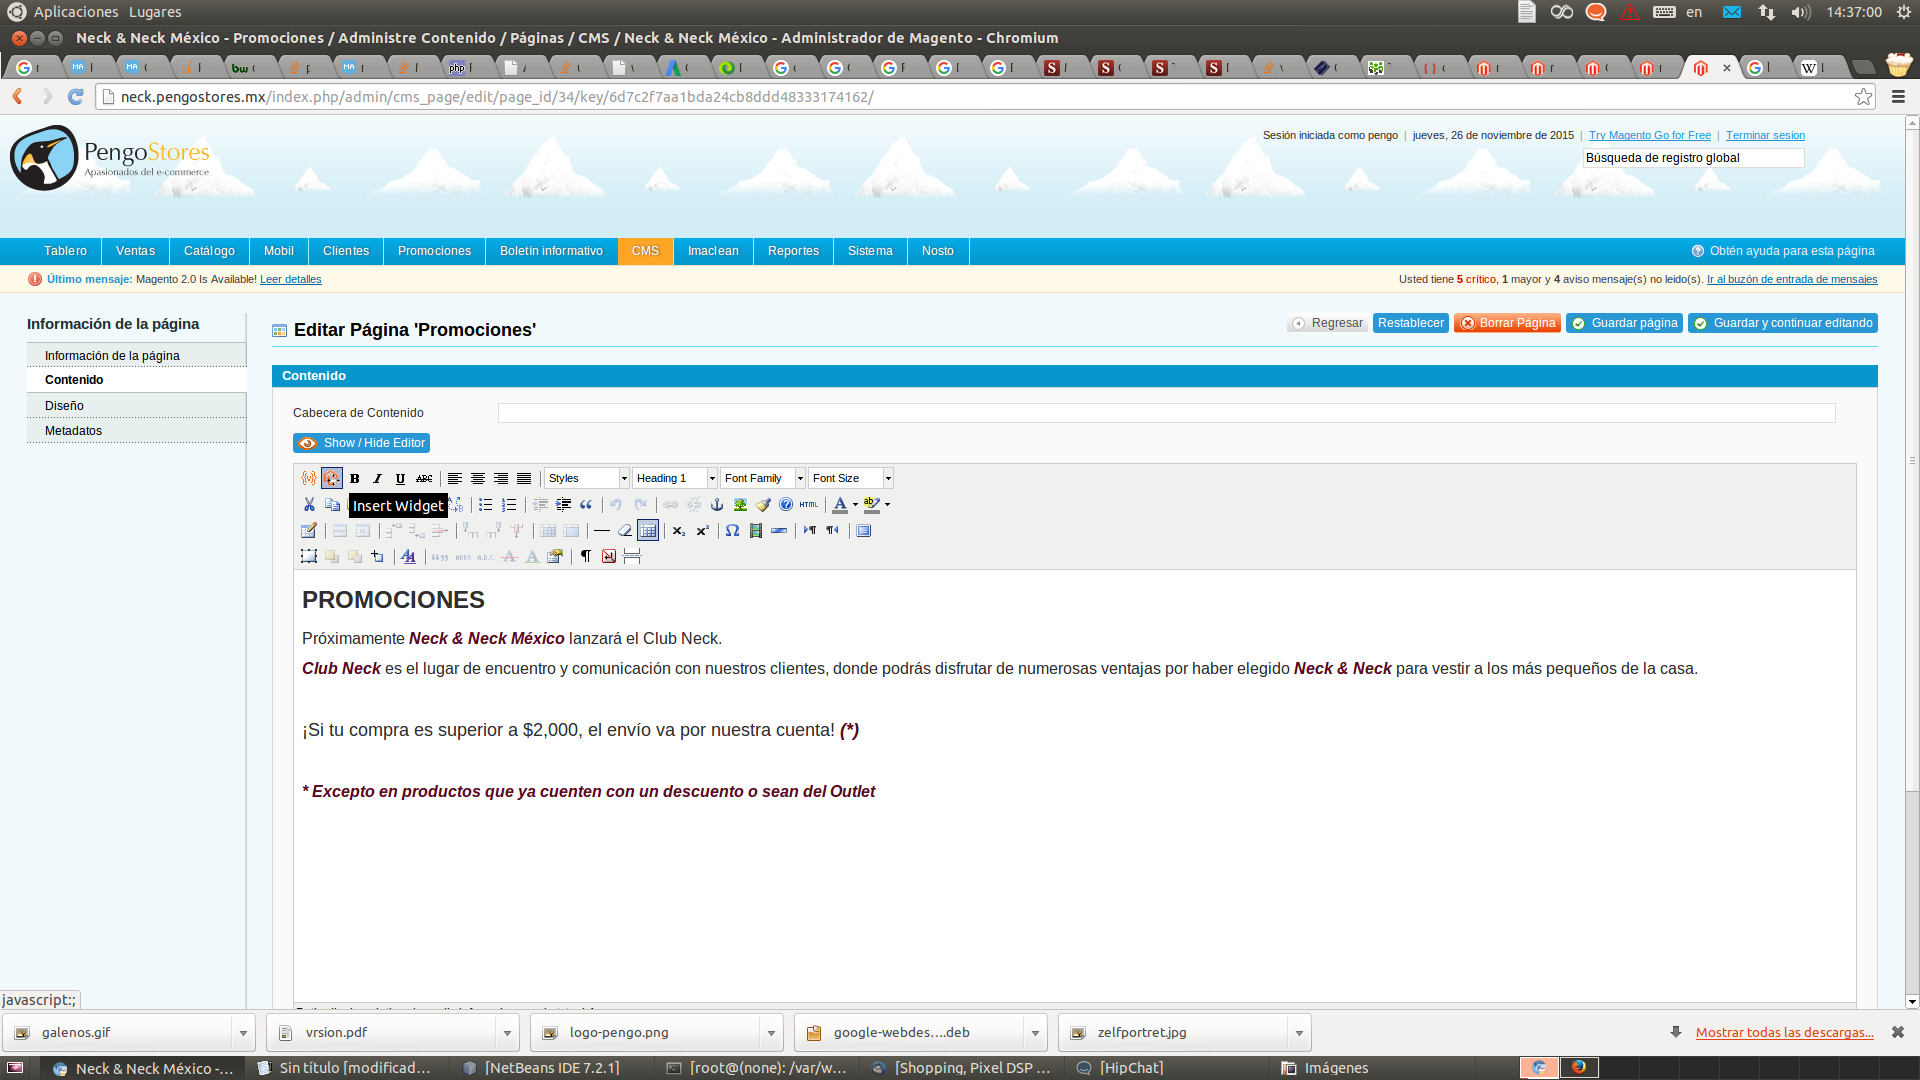
\includegraphics[width=16cm]{widget001}
\caption{pantalla Verificar}
\label{fig:flat}
\end{figure}

\subsection{Paso 3}

Para el Paso 3 

Ventajas de Usar Videowidget

}



\begin{enumerate}
\setcounter{enumi}{3}
\item Puede Ir en cualquier parte de un Bloque Estatico.
\item Puede Ir en cualquier Pagina Estatica.
\item Puede ser llamado en un Template \cite{magento}.
\item Algunos Pueden ir en Correos transaccionales ?.
\end{enumerate}

\begin{center}
\begin{figure}[htp]
\centering
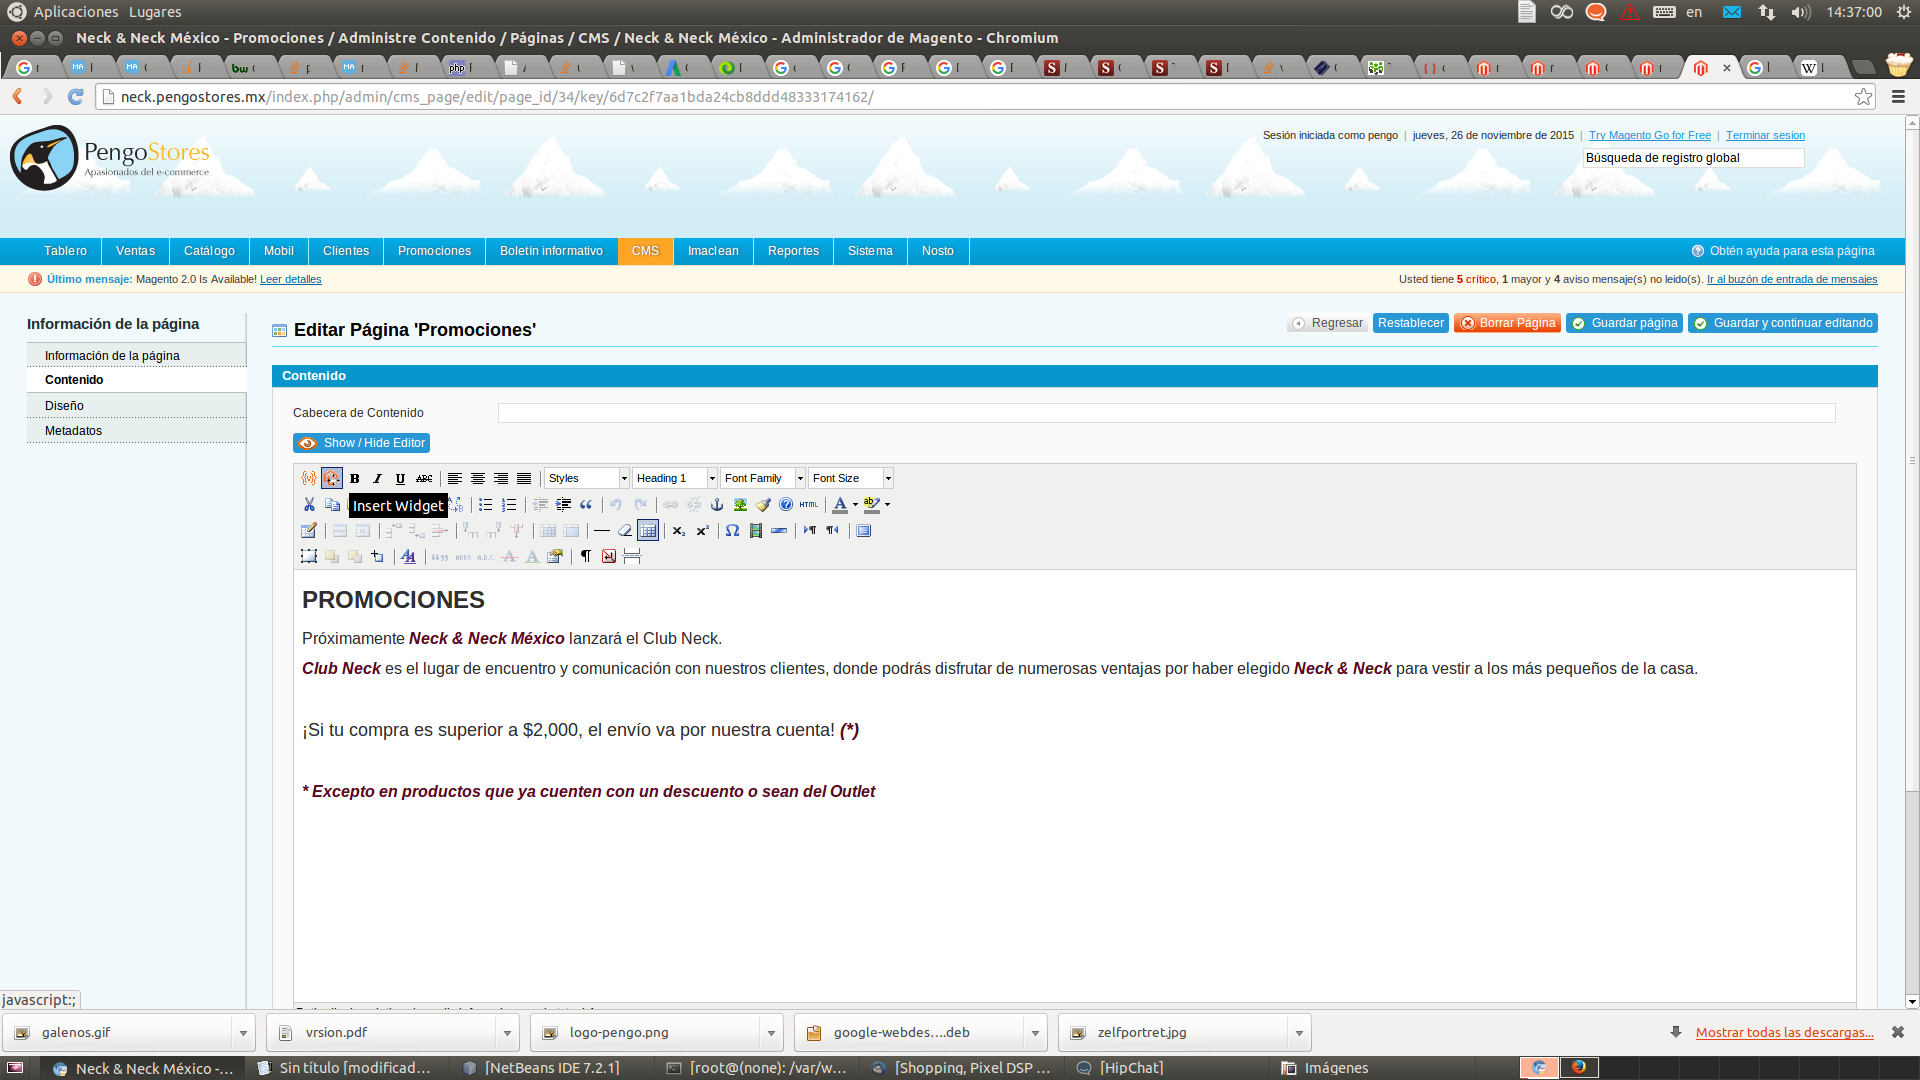
\includegraphics[width=16cm]{widget00}
\caption{pantalla Revisa Url}
\label{fig:super}
\end{figure}
\end{center}



Para el final del Modulo 



\import{sections/}{out.tex}


\begin{thebibliography}{9}
\bibitem{latexcompanion} 
Modulo Pengo CMS. 
\textit{Pengo Manuales}. 
Adrian Romero Vargas, Francisco Espinosa, Mayra Caballero, Version 1.
 
\bibitem{magento} 
Magento Inc. 
\textit{Magento Enterprise Documentation}. (Ingles) 
[\textit{Magento CMC and Widget}]. 
Documentation,Magento Enterprise, 2013.
 
\bibitem{magentoconnect} 
Magento Connect,
\\\texttt{http://www.magento.com/connect/widget.html}
\end{thebibliography}


\end{document}
